\documentclass[12pt,a4paper,oneside]{article}

\usepackage[margin=0.9in]{geometry}
\usepackage[utf8]{inputenc}
\usepackage{graphicx}
\usepackage{amsmath}
\usepackage{amsfonts}
\usepackage{amssymb}
\usepackage{graphicx}
\usepackage{multirow}
\usepackage{color}
\usepackage{xcolor}
\usepackage{url}
\usepackage{enumerate}
\usepackage{lastpage}
\usepackage{tikz}

\usepackage{fancyhdr}
\pagestyle{fancy}
\lhead{\textbf{CPSE:SF LU WS2016/17}}
\rhead{EXERCISE 2}
\cfoot{\thepage\ of \pageref{LastPage}}
\renewcommand{\headrulewidth}{0.4pt}
\renewcommand{\footrulewidth}{0.4pt}

\sloppy

\usepackage{subfig}
\usepackage{listings}
\lstset{
language=Matlab,
basicstyle=\tiny,
numbers=left,
numberstyle=\tiny\color{gray},
stepnumber=5,
numbersep=5pt,
showstringspaces=false,
frame=single,
captionpos=b,
breaklines=true,
keywordstyle=\color{blue},
commentstyle=\color{dkgreen},
stringstyle=\color{mauve},
}

\usepackage{etoolbox}
\let\bbordermatrix\bordermatrix
\patchcmd{\bbordermatrix}{8.75}{4.75}{}{}
\patchcmd{\bbordermatrix}{\left(}{\left[}{}{}
\patchcmd{\bbordermatrix}{\right)}{\right]}{}{}



\newcommand{\answer}[1]{{\color{dkgreen} #1 } }
\newcommand{\comment}[1]{{\color{blue} #1 } }

\begin{document}
\setcounter{MaxMatrixCols}{20}
\newcommand{\fcl}[1]{{\footnotesize#1\vspace{0.4cm}\\}}
\newcommand{\fclc}[2]{{\footnotesize#1\hspace{0.4cm}{\footnotesize #2}\vspace{0.4cm}}\\}
\newcommand{\mmatrix}[1]{\left [ \begin{matrix}#1\end{matrix} \right ]}
\newcommand{\SpaceEx}[0]{\textsc{SpaceEx} }

%% vector
\newcommand{\vc}[1]{\ensuremath{\boldsymbol{\lowercase{#1}}}}

%% matrix
\newcommand{\mt}[1]{\ensuremath{\boldsymbol{\uppercase{#1}}}}

%% random vector
\newcommand{\rvc}[1]{\ensuremath{\text{\sffamily\bfseries\lowercase{#1}}}}

%% random matrix
\newcommand{\rmt}[1]{\ensuremath{\text{\sffamily\bfseries\uppercase{#1}}}}

%% random variable
\newcommand{\rv}[1]{\ensuremath{\text{\sffamily\lowercase{#1}}}}


%\newcommand{\rv}[1]{\mathrm{#1}}
%\newcommand{\rvv}[1]{\bm{\mathrm{#1}}}
\newcommand{\dv}[1]{\mathit{#1}}
\newcommand{\dvv}[1]{\bm{\mathit{#1}}}
\newcommand{\pdf}[1]{f_\rv{#1}(\dv{#1})}
\newcommand{\pdfa}[2]{f_\rv{#1}(\dv{#2})}
%\newcommand{\cdf}[1]{F_\rv{#1}(\dv{#1})}
\newcommand{\cdf}[2]{F_\rv{#1}(\dv{#2})}
\newcommand{\prob}[1]{\mathrm{P}\{#1\}}
\newcommand{\pmf}[1]{p_\rv{#1}(\dv{#1})}

% -------------------------------------------------------------------
%
% YOUR SUBMISSION
% - uncomment and fill the group information below
% - you can remove the "Important"-paragraph
%
% -------------------------------------------------------------------

%% \title{
%%   Cyber-Physical Systems Engineering:\\Stochastic Foundations LU WS2016/17 \\
%%   \textbf{Exercise 2}
%% }
%% \author{
%%   {\bf Group X} \vspace{0.2cm}\\
%%   .. group members .. \\
%% }
%% \date{18.11.2016}
%% \maketitle

\paragraph{Important}
\begin{itemize}
  \item Completeness of solution: A complete solution of a task also
    includes knowledge about the theory behind. This will be checked
    during the exercise meeting.
  \item Grading: 10 points per exercise, distributed among up to 4
    tasks per exercise. Presence during exercise discussion
    mandatory. No deadline extensions.
  \item Collaboration: Exercises may be solved in groups. However, {\bf every}
    group member must be able to explain the handed in solution. Grading is on
    an individual basis.
  \item Deliverables: Please upload your solution (one per group) to
    TUWEL until {\bf 16.11.2016, 23:55}.
  \item Next exercises meeting: 18.11.2016 10:00 (c.t.), TI SEM.
\end{itemize}


%
% --- T2.1 ----------------------------------------------------------%
%
\subsubsection*{Task 2.1: Conditional Independence in Bayes Nets, 1 point}
\begin{figure}[ht]
  \centering
  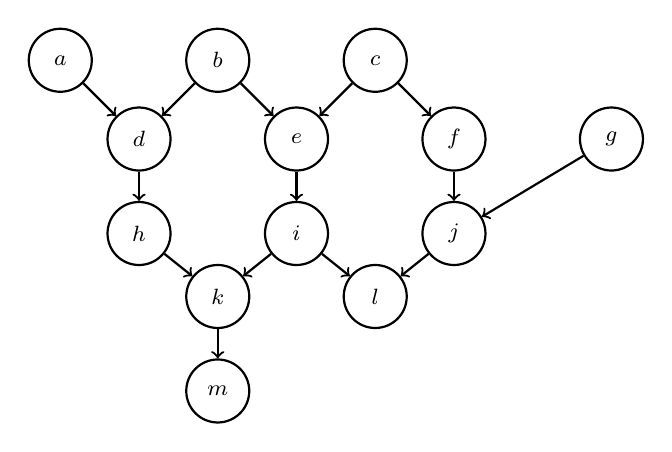
\begin{tikzpicture}[node distance=3.1cm,auto]
    \tikzstyle{every node}=[shape=circle,minimum size=8mm,font=\footnotesize];
    \tikzstyle{every path} = [draw,thick];

    \node (A) [draw] at (1,5) {$\rv{a}$};
    \node (B) [draw] at (3,5) {$\rv{b}$};
    \node (C) [draw] at (5,5) {$\rv{c}$};
    \node (D) [draw] at (2,4) {$\rv{d}$};
    \node (E) [draw] at (4,4) {$\rv{e}$};
    \node (F) [draw] at (6,4) {$\rv{f}$};
    \node (G) [draw] at (8,4) {$\rv{g}$};
    \node (H) [draw] at (2,2.8) {$\rv{h}$};
    \node (I) [draw] at (4,2.8) {$\rv{i}$};
    \node (J) [draw] at (6,2.8) {$\rv{j}$};
    \node (K) [draw] at (3,2) {$\rv{k}$};
    \node (L) [draw] at (5,2) {$\rv{l}$};
    \node (M) [draw] at (3,0.8) {$\rv{m}$};

    \path[->] (A) edge node {} (D);
    \path[->] (B) edge node {} (D);
    \path[->] (B) edge node {} (E);
    \path[->] (C) edge node {} (E);
    \path[->] (C) edge node {} (F);
    \path[->] (D) edge node {} (H);
    \path[->] (E) edge node {} (I);
    \path[->] (F) edge node {} (J);
    \path[->] (G) edge node {} (J);
    \path[->] (H) edge node {} (K);
    \path[->] (I) edge node {} (K);
    \path[->] (I) edge node {} (L);
    \path[->] (J) edge node {} (L);
    \path[->] (K) edge node {} (M);
  \end{tikzpicture}
  \caption{A Bayesian network.}
  \label{fig:bn1}
\end{figure}

\begin{enumerate}[a)]
\item Considering the Bayes net in Figure \ref{fig:bn1}, which statements are
  true?

  \vspace{0.2cm}
  \begin{tabular}{|l|l|}
    \hline
    $\rv{a} \perp \rv{k}$ & \hspace{1cm} \\ \hline
    $\rv{a} \perp \rv{k} \; | \; \rv{d}$ & \hspace{1cm} \\ \hline
    $\rv{a} \perp \rv{k} \; | \; \rv{h}$ & \hspace{1cm} \\ \hline
    $\rv{h} \perp \rv{i}$ & \\ \hline
  \end{tabular}
  \hspace{0.2cm}
  \begin{tabular}{|l|l|}
    \hline
    $\rv{h} \perp \rv{i} \; | \; \rv{b}$ & \hspace{1cm} \\ \hline
    $\rv{a} \perp \rv{l} \; | \; \rv{b}, \rv{m}$ & \\ \hline
    $\rv{a} \perp \rv{g}$ & \\ \hline
    $\rv{d} \perp \rv{g} \; | \; \rv{e}, \rv{l}$ & \\ \hline
  \end{tabular}
  \vspace{0.2cm}
\end{enumerate}


%
% --- T2.2 ----------------------------------------------------------%
%
\subsubsection*{Task 2.2: Inference in Bayes Nets, 4 points}

A drone is flying at an altitude that is modelled by the random variable
$\rv{a}$.  Two sensors measure the altitude. The measurements are modelled by
the random variable $\rv{m}_1$ and respectively the random variable $\rv{m}_2$.
With a probability of $\epsilon$ the measurement is incorrect by
$1m$. Additionally, each sensor can be (with a probability $f$) badly
miscalibrated (modelled by random variables $\rv{c}_1$ and respectively
$\rv{c}_2$) and constantly report an altitude that is at least $3m$ lower than
the actual altitude.  Hence, in case a sensor is badly miscalibrated and the
altitude is less than $3m$ the sensor will report an altitude of zero.

\begin{figure}[ht]
  \centering
  \subfloat[]{
    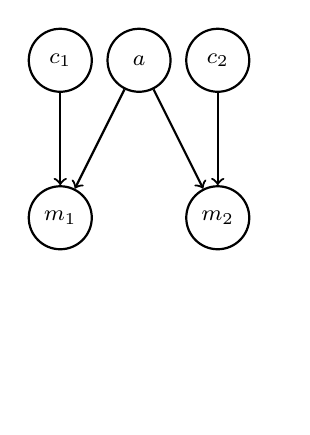
\begin{tikzpicture}[node distance=3.1cm,auto]
      \tikzstyle{every node}=[shape=circle,minimum size=8mm,font=\footnotesize];
      \tikzstyle{every path} = [draw,thick];

      \node (C1) [draw] at (0,4) {$\rv{c}_1$};
      \node (C2) [draw] at (2,4) {$\rv{c}_2$};
      \node (M1) [draw] at (0,2) {$\rv{m}_1$};
      \node (M2) [draw] at (2,2){$\rv{m}_2$};
      \node (N) [draw] at (1,4) {$\rv{a}$};
      \node at (0,0) {};

      \path[->] (C1) edge node {} (M1);
      \path[->] (C2) edge node {} (M2);
      \path[->] (N) edge node {} (M1);
      \path[->] (N) edge node {} (M2);
    \end{tikzpicture}

  }
  \subfloat[]{
    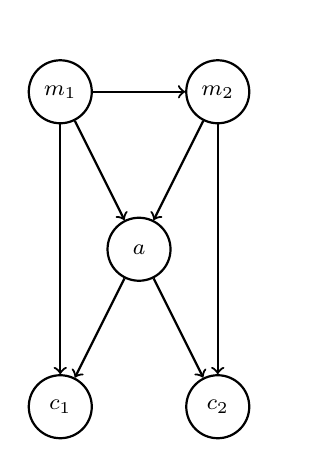
\begin{tikzpicture}[node distance=3.1cm,auto]
      \tikzstyle{every node}=[shape=circle,minimum size=8mm,font=\footnotesize];
      \tikzstyle{every path} = [draw,thick];

      \node (C1) [draw] at (0,0) {$\rv{c}_1$};
      \node (C2) [draw] at (2,0) {$\rv{c}_2$};
      \node (M1) [draw] at (0,4) {$\rv{m}_1$};
      \node (M2) [draw] at (2,4){$\rv{m}_2$};
      \node (N) [draw] at (1,2) {$\rv{a}$};

      \path[->] (M1) edge node {} (C1);
      \path[->] (M2) edge node {} (C2);
      \path[->] (N) edge node {} (C1);
      \path[->] (N) edge node {} (C2);
      \path[->] (M1) edge node {} (N);
      \path[->] (M2) edge node {} (N);
      \path[->] (M1) edge node {} (M2);
    \end{tikzpicture}

  }
  \subfloat[]{
    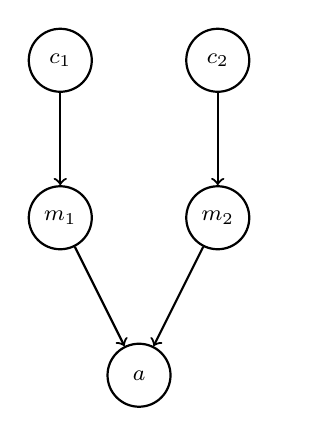
\begin{tikzpicture}[node distance=3.1cm,auto]
      \tikzstyle{every node}=[shape=circle,minimum size=8mm,font=\footnotesize];
      \tikzstyle{every path} = [draw,thick];

      \node (C1) [draw] at (0,4) {$\rv{c}_1$};
      \node (C2) [draw] at (2,4) {$\rv{c}_2$};
      \node (M1) [draw] at (0,2) {$\rv{m}_1$};
      \node (M2) [draw] at (2,2){$\rv{m}_2$};
      \node (N) [draw] at (1,0) {$\rv{a}$};

      \path[->] (C1) edge node {} (M1);
      \path[->] (C2) edge node {} (M2);
      \path[->] (M1) edge node {} (N);
      \path[->] (M2) edge node {} (N);
    \end{tikzpicture}

  }
  \subfloat[]{
    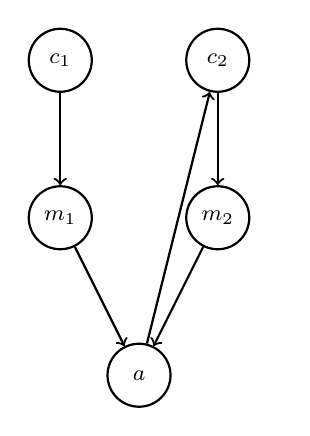
\begin{tikzpicture}[node distance=3.1cm,auto]
      \tikzstyle{every node}=[shape=circle,minimum size=8mm,font=\footnotesize];
      \tikzstyle{every path} = [draw,thick];

      \node (C1) [draw] at (0,4) {$\rv{c}_1$};
      \node (C2) [draw] at (2,4) {$\rv{c}_2$};
      \node (M1) [draw] at (0,2) {$\rv{m}_1$};
      \node (M2) [draw] at (2,2){$\rv{m}_2$};
      \node (N) [draw] at (1,0) {$\rv{a}$};

      \path[->] (C1) edge node {} (M1);
      \path[->] (C2) edge node {} (M2);
      \path[->] (M1) edge node {} (N);
      \path[->] (M2) edge node {} (N);
      \path[->] (N) edge node {} (C2);
    \end{tikzpicture}
  }
  \caption{Several Bayes nets of measuring the altitude of a drone.}
  \label{fig:altitude}
\end{figure}

\begin{enumerate}[a)]
\item What independence claims (e.g., $a \perp b \; | \; c$, $d \perp e$) can
  you make considering the hypothesis above?
\item Consider the graphs in Figure~\ref{fig:altitude}. Which of them
  represents the given information correctly (but not necessarily efficiently)
  as a Bayesian network?
\item Which of the networks is the best representation? Why?
\item Give the conditional distribution for $P(\rv{m}_1|\rv{a})$ for the case
  where $\rv{a}\in\{1,2,3\}$ and $\rv{m}_1\in\{0,1,2,3,4\}$. All entries of the
  conditional distribution table (CPT) should be written as a function of the
  parameters $\epsilon$ and/or $f$ (e.g., $P(\rv{m}_1=0|\rv{a}=3)=f$).
\item Assume that the two sensors work identically. $a \in \{1, 2, 3\}$ and
  $m_1, m_2 \in \{0, 1, 2, 3, 4\}$, with the symbolic CPTs as described
  above. Using the variable elimination algorithm, calculate the probability
  distribution $P(\rv{a} | \rv{m}_1 = 2, \rv{m}_2 = 2)$.
\item Explain the advantages of \emph{variable elimination} over naive
  enumeration.
\end{enumerate}


%
% --- T2.3 ----------------------------------------------------------%
%
\subsubsection*{Task 2.3: Conditional Independence and Sampling in Bayes Nets, 2 points}
Suppose that in a Bayesian network containing an unobserved variable $\rv{x}$,
all the variables in the Markov blanket $MB(\rv{x})$ have been observed.
%
The \emph{Markov blanket} of a node $\rv{x}$ is a set of nodes including the
parents, children and children's parents of $\rv{x}$.

\begin{enumerate}[a)]
\item Prove that a variable $\rv{x}$ is conditionally independent of all other
  variables in the network given its Markov blanket $MB(\rv{x})$.
\item Discuss whether we can remove $\rv{x}$ if we are planning to use
  (i)~rejection sampling and (ii)~likelihood weighting.
\end{enumerate}

%
% --- T2.4 ----------------------------------------------------------%
%
\subsubsection*{Task 2.4: Matlab Introduction, 3 points}
A heater element and its environment are modeled according to the Simulink
continuous-time model in Figure~\ref{fig:heat}. The output is in degree
Celsius, the input is a real value between zero (don't heat) and one (apply
max. heat). The delay of the 'Transport Delay' block is 30 seconds.
%\begin{figure}[htb]
%  \centering
%  \includegraphics[width=0.7\textwidth]{t24}
%  \caption{Task 3.1, Plant Model}
%  \label{fig:heat}
%\end{figure}

\begin{enumerate}[a)]
\item Do a step-response analysis and determine PID controller parameters by
  applying the Ziegler–Nichols
  method~\footnote{\url{https://en.wikipedia.org/wiki/PID_controller}}.  Also
  include a plot of the step-response function in your deliverable.
\item Build a negative-feedback PID controlled system that includes the modeled
  plant and plot the system reaction to a few simple set-point input functions
  (step, multi-step, sin,~\ldots).
\end{enumerate}


\end{document}
